% CVPR 2027 submission, built on the CVPR 2026 author kit (https://github.com/cvpr-org/author-kit).
% Replace cvpr.sty / ieeenat_fullname.bst with the official 2027 kit once it is released.

\documentclass[10pt,twocolumn,letterpaper]{article}

%%%%%%%%% PAPER TYPE  - PLEASE UPDATE FOR FINAL VERSION
% \usepackage{cvpr}              % To produce the CAMERA-READY version
\usepackage[review]{cvpr}      % To produce the REVIEW version
% \usepackage[pagenumbers]{cvpr} % To force page numbers, e.g. for an arXiv version

% preamble.tex loads hyperref; pass its options before that first load.
\definecolor{cvprblue}{rgb}{0.21,0.49,0.74}
\PassOptionsToPackage{pagebackref,breaklinks,colorlinks,allcolors=cvprblue}{hyperref}
%% Packages and layout tweaks, loaded by main.tex and rebuttal.tex before hyperref.
%%
%% Already loaded by cvpr.sty -- do NOT load again (option clashes):
%%   times, xspace, xcolor[dvipsnames], graphicx, amsmath, amssymb, booktabs,
%%   natbib, caption, subcaption, url, etoolbox, enumitem, cleveref (after hyperref)
%% Project macros (notes, method name, notation, table helpers) live in macros.tex.

%% ---------------------------------------------------------------------------
%% Packages
%% ---------------------------------------------------------------------------
\usepackage{multirow}    % \multirow in tables
\usepackage{tabularx}    % X columns that fill \linewidth
\usepackage{lipsum}
\usepackage{booktabs}
\usepackage{amsmath}
\usepackage{makecell}
\usepackage{array} 
\usepackage{colortbl}    % \rowcolor / \cellcolor (xcolor is already loaded)
\usepackage{bm}          % bold math symbols, \bm{x}
\usepackage{pifont}
\usepackage{amssymb}    
% \ding symbols for \cmark / \xmark
\usepackage{color}
\usepackage{colortbl}
\usepackage{subcaption}
% Uncomment if needed:
% \usepackage{algorithm}
% \usepackage{algpseudocode}
% \usepackage{wrapfig}
% \usepackage{siunitx}   % aligned numeric columns, e.g. S[table-format=2.1]
\DeclareMathOperator*{\argtopk}{arg\,top-K}

% \newcommand{\red}[1]{{\color{red}#1}}
\newcommand{\orange}[1]{{\color{orange}#1}}
\newcommand{\blue}[1]{{\color{cyan}#1}}
\newcommand{\gray}[1]{{\color{gray}#1}}
%% ---------------------------------------------------------------------------
%% Paths
%% ---------------------------------------------------------------------------
\newcommand{\paragrapht}[1]{\noindent\textbf{#1}} 
\graphicspath{{figures/}}

% \newcommand{\cmark}{\ding{51}}%
% \newcommand{\xmark}{\ding{55}}%

\newcommand\blfootnote[1]{%
  \begingroup
  \renewcommand\thefootnote{}\footnote{#1}%
  \addtocounter{footnote}{-1}%
  \endgroup
}

\usepackage{xspace}
% \usepackage{multirow}
\usepackage{array}
\usepackage{layouts}
\usepackage{algorithm}
\usepackage{bbding}
\usepackage{listings}
\usepackage{pifont}
\usepackage{wasysym}
\usepackage{float}
\usepackage{soul}
\usepackage{footnote}
\makesavenoteenv{tabular}
\makesavenoteenv{table}
\makesavenoteenv{figure}
\usepackage{pythonhighlight}
\usepackage{enumitem}
\usepackage{graphicx}
\usepackage{wrapfig}
\usepackage{bbm}

\usepackage{hyperref}
\usepackage[capitalize,noabbrev]{cleveref}
\usepackage{tikz}
\usepackage{threeparttable}
\usetikzlibrary{patterns,patterns.meta}

\newcommand{\ji}[1]{\textcolor{blue}{#1}}
\newcommand{\cj}[1]{\textcolor{magenta}{#1}}

%% ---------------------------------------------------------------------------
%% Layout tweaks -- enable only near the end, when fighting the page limit
%% ---------------------------------------------------------------------------
% Tighter text layout (typically saves ~1/6 page):
% \usepackage{microtype}

% Compact run-in paragraph headings:
% \renewcommand{\paragraph}[1]{\vspace{.5em}\noindent\textbf{#1.}}

% Less space between figure and caption:
% \setlength{\abovecaptionskip}{.5em}

% Less space around floats:
% \setlength{\textfloatsep}{10pt plus 2pt minus 2pt}
% \setlength{\dbltextfloatsep}{10pt plus 2pt minus 2pt}

% Tighter underline:
% \usepackage{soul}
% \setuldepth{foobar}

\usepackage{hyperref}

% Project macros: draft notes, method name, notation, table helpers
%% Project macros, loaded after hyperref by main.tex and rebuttal.tex.

%% ===========================================================================
%% Draft switch: set \draftfalse before submission -- every \TODO and \note
%% disappears and \todo / \red text turns black.
%% ===========================================================================
\newif\ifdraft
\drafttrue

\ifdraft
  \newcommand{\TODO}[1]{\textbf{\color{red}[TODO: #1]}}   % missing content
  \newcommand{\todo}[1]{{\color{red}#1}}                  % text that needs revision
  \newcommand{\red}[1]{{\color{red}#1}}
  \newcommand{\note}[2]{{\color{blue}[\textbf{#1}: #2]}}  % \note{YW}{comment}
\else
  \newcommand{\TODO}[1]{}
  \newcommand{\todo}[1]{#1}
  \newcommand{\red}[1]{#1}
  \newcommand{\note}[2]{}
\fi

%% ===========================================================================
%% Names (rename in one place)
%% ===========================================================================
\newcommand{\method}{ARROW\xspace}

%% ===========================================================================
%% Notation
%% ===========================================================================
\newcommand{\R}{\mathbb{R}}
\newcommand{\E}{\mathbb{E}}
\DeclareMathOperator*{\argmin}{arg\,min}
\DeclareMathOperator*{\argmax}{arg\,max}
\newcommand{\norm}[1]{\left\lVert#1\right\rVert}
\newcommand{\abs}[1]{\left\lvert#1\right\rvert}

%% ===========================================================================
%% Tables
%% ===========================================================================
\newcommand{\cmark}{\ding{51}}                              % check mark
\newcommand{\xmark}{\ding{55}}                              % cross
\newcommand{\best}[1]{\textbf{#1}}
\newcommand{\second}[1]{\underline{#1}}
\newcommand{\gain}[1]{{\scriptsize\color{ForestGreen}(+#1)}} % \gain{4.6}
\newcommand{\drop}[1]{{\scriptsize\color{BrickRed}(-#1)}}    % \drop{3.0}
\newcommand{\pp}{\,pp\xspace}                                % percentage points
\newcommand{\oursrow}{\rowcolor{cvprblue!8}}                 % shade "ours" rows

%% ===========================================================================
%% Figures: gray box with the final size, until the real figure exists.
%%   \placeholder{3cm}                 -> full column width, 3 cm tall
%%   \placeholder[0.48\linewidth]{3cm} -> custom width
%% ===========================================================================
\newcommand{\placeholder}[2][\linewidth]{%
  \fbox{\parbox[c][#2][c]{\dimexpr #1-2\fboxsep-2\fboxrule\relax}%
    {\centering\small\color{gray}placeholder}}}


%%%%%%%%% PAPER ID  - PLEASE UPDATE
\def\paperID{*****} % *** Enter the Paper ID here
\def\confName{CVPR}
\def\confYear{2027}

%%%%%%%%% TITLE - PLEASE UPDATE
\title{ARROW: Action-Aware Resolution Routing for World Action Models}

%%%%%%%%% AUTHORS - PLEASE UPDATE (hidden automatically in review mode)
\author{First Author\\
Institution1\\
{\tt\small firstauthor@i1.org}
\and
Second Author\\
Institution2\\
{\tt\small secondauthor@i2.org}
}

\begin{document}

%%%%%%%%% TITLE (+ OPTIONAL FULL-WIDTH TEASER)
% Default: plain title. For a full-width teaser under the title, comment out
% \maketitle and uncomment the block below (put the image in figures/).
\maketitle
% \twocolumn[{%
%   \renewcommand\twocolumn[1][]{#1}%
%   \maketitle
%   \begin{center}
%     \centering
%     \includegraphics[width=\linewidth]{teaser}
%     \captionof{figure}{Teaser caption.}
%     \label{fig:teaser}
%   \end{center}%
%   \vspace{1em}
% }]

%%%%%%%%% MAIN PAPER (8 pages, references excluded)
\begin{abstract}
    \ji{
    World action models (WAMs) have emerged as a promising approach to robotic control by jointly modeling future visual dynamics and actions. 
    However, the dense spatiotemporal representations required for video generation introduce substantial computational overhead, even though not all visual information is equally relevant to action prediction. 
    In this paper, we propose \method, an efficient WAM framework that allocates computation according to the action relevance of future visual representations. 
    Our key idea is to preserve fine-grained spatiotemporal information where it matters for action generation, while representing less relevant regions at coarser resolutions. 
    To this end, we introduce a lightweight action-aware router trained with gradient-based supervision from the action decoder. 
    The learned relevance guides spatial token merging, preserving the resolution of action-critical regions, while adaptive temporal aggregation jointly considers action relevance and feature dynamics to capture their temporal evolution. 
    We further employ velocity distillation to adapt the action decoder to compressed representations without updating the video generation backbone.
    By selectively allocating spatial and temporal resolution, \method reduces the number of future tokens by up to 90\% in the specified configuration.
    [Quantitative results demonstrating action performance and inference efficiency.]
    }
% World action models (WAMs) build robot policies on pretrained video generation models, so that the action decoder inherits the visual and dynamic knowledge of the video backbone.
% The backbone, however, processes a dense spatio-temporal token grid whose layout is set by video generation, while the action decoder relies on only part of it;
% the rest is redundant for control but is still computed and passed to the decoder.
% Generic token reduction does not resolve this mismatch:
% visual similarity is a poor proxy for action relevance, and deleting tokens degrades the policy sharply when few tokens are kept.
% We propose \method, an action-aware token allocation that lets the action, rather than visual content, decide where and at which resolution the video backbone computes.
% A lightweight router, supervised only by how each token affects the predicted action, scores the future-frame tokens.
\end{abstract}

\section{Introduction}
\label{sec:intro}

% ---- 脉络--------------------------------------------------------
% P1  World action model（WAM）：用预训练视频生成模型做 backbone，policy 继承世界知识与动态先验。
% P2  代价与矛盾：backbone 的 token 空间由生成目标决定（稠密、均匀的时空网格），
%     而 action head 只需要其中一小部分；推理成本跟着生成形状走，而不是跟着控制需要走。
% P3  为什么现成的 token 剪枝在 WAM 的部署点上不成立：
%     相似度 != 冗余（future 帧近似噪声占位）；删除会破坏 backbone 的结构；
%     空间与时间两个轴的位置约定相反。
% P4  观点：应由 action 而不是视觉内容决定 backbone 在哪里、以什么分辨率计算
%     （在常规的 video -> action 之外，加上 action -> video 的通路）。
% P5  方法一段：C1 action-aware router；C2 空间分辨率分配（合并而非删除）；
%     C3 router 引导的时间分辨率 + 紧凑时间位置；可 fold 的 decoder 适配。
% P6  结果一句（对 native 只能写"不可区分"，不能写"超过"）。
% 贡献列表：C1 / C2 / C3（分析部分作为动机，不另算）。
% 若用 teaser：main.tex 中有整栏 teaser 的写法，label 为 fig:teaser。
% ---------------------------------------------------------------------------

% ---- 数字来源与措辞边界（Claude 起草时记录）----------------------------------
% 写法：由一般到具体逐步收窄，P2、P3 末尾用陈述句点出问题（intro 中不用疑问句），P4 隐晦地指向方法；正文不出现具体模型名。
% 引用共 4 篇：pai2025mimicvideo、ye2026dreamzero（提出 "world action model" 一词）、bolya2023tome、liu2023libero，均已在 main.bib 中。
% 只引用已写的 Sec. 4 与 fig:overview。Sec. 3 已删除，P3 的论断（相似度不等于动作相关、删除会丢掉场景）需在 Sec. 5 给出依据。
% P6 数字（LIBERO，每个套件 n=500，逐 episode 配对 exact McNemar；预算只作用于 16,800 个 future token，
%   2,400 个 observation token 全部保留）：20% future（总 5,760 = 30%）Spatial 441 vs 452（p=0.22），
%   Object 470 vs 470（p=1），Goal 447 vs 451（p=0.71）-> 只写"不可区分"。Object 的冻结 router 配方不同，Sec. 5 需注明。
% "necessary for the policy"：E1 反转排序（Spatial），20% -22.0pp、10% -42.4pp，Holm p<=6e-21。
% "concentrate on the robot and the objects"：E3（Spatial）满分辨率组覆盖任务物体像素 90%、机械臂 84%、背景 26%（随机 33%）；
%   不能写"按指令选择"。
% adapter 可 fold：闭环核查只在旧算子上做过（合并 -1.10pp，p=0.15），定稿算子上尚未复核。
% 第二个 backbone（DiT4DiT）按"暂不提具体模型名"的要求不放 intro；DeVA 不在论文中出现。
% P4 讨论 decoder attention 的利弊：只从"时机"（要先算完全分辨率的 future）和"度量的量不同"两点论证，
%   不说 router 优于 decoder attention——E2 离线中完整上下文的 decoder cross-attention 比 router 好 7%（p=0.0078）。
% ---------------------------------------------------------------------------

Large video generation models, trained on vast amounts of video, capture how the visual world looks and how it changes over time.
World action models (WAMs)~\cite{pai2025mimicvideo,ye2026dreamzero} bring this knowledge to robot control:
a pretrained video model predicts how the scene will evolve under an instruction, and the robot's actions are derived from this predicted future,
typically by an action decoder that reads the internal representation of the video model.
Such policies inherit visual and physical priors from video pretraining, rather than learning them from robot demonstrations alone.

A video model, however, is built to generate video.
Its representation of the future covers every region of every frame on a dense, uniform grid, because generation must render the entire scene.
Acting in the scene asks for something narrower: the next actions depend mostly on the robot, the objects it interacts with, and the space it is about to move through.
Yet the action decoder receives the full, generation-shaped representation, and the video model computes all of it at full resolution, regardless of which parts the action actually uses.
Whether a policy needs the predicted future at the resolution at which it would be generated, and which parts of it the action actually relies on, has so far received little attention.

\begin{figure}[t]
  \centering
  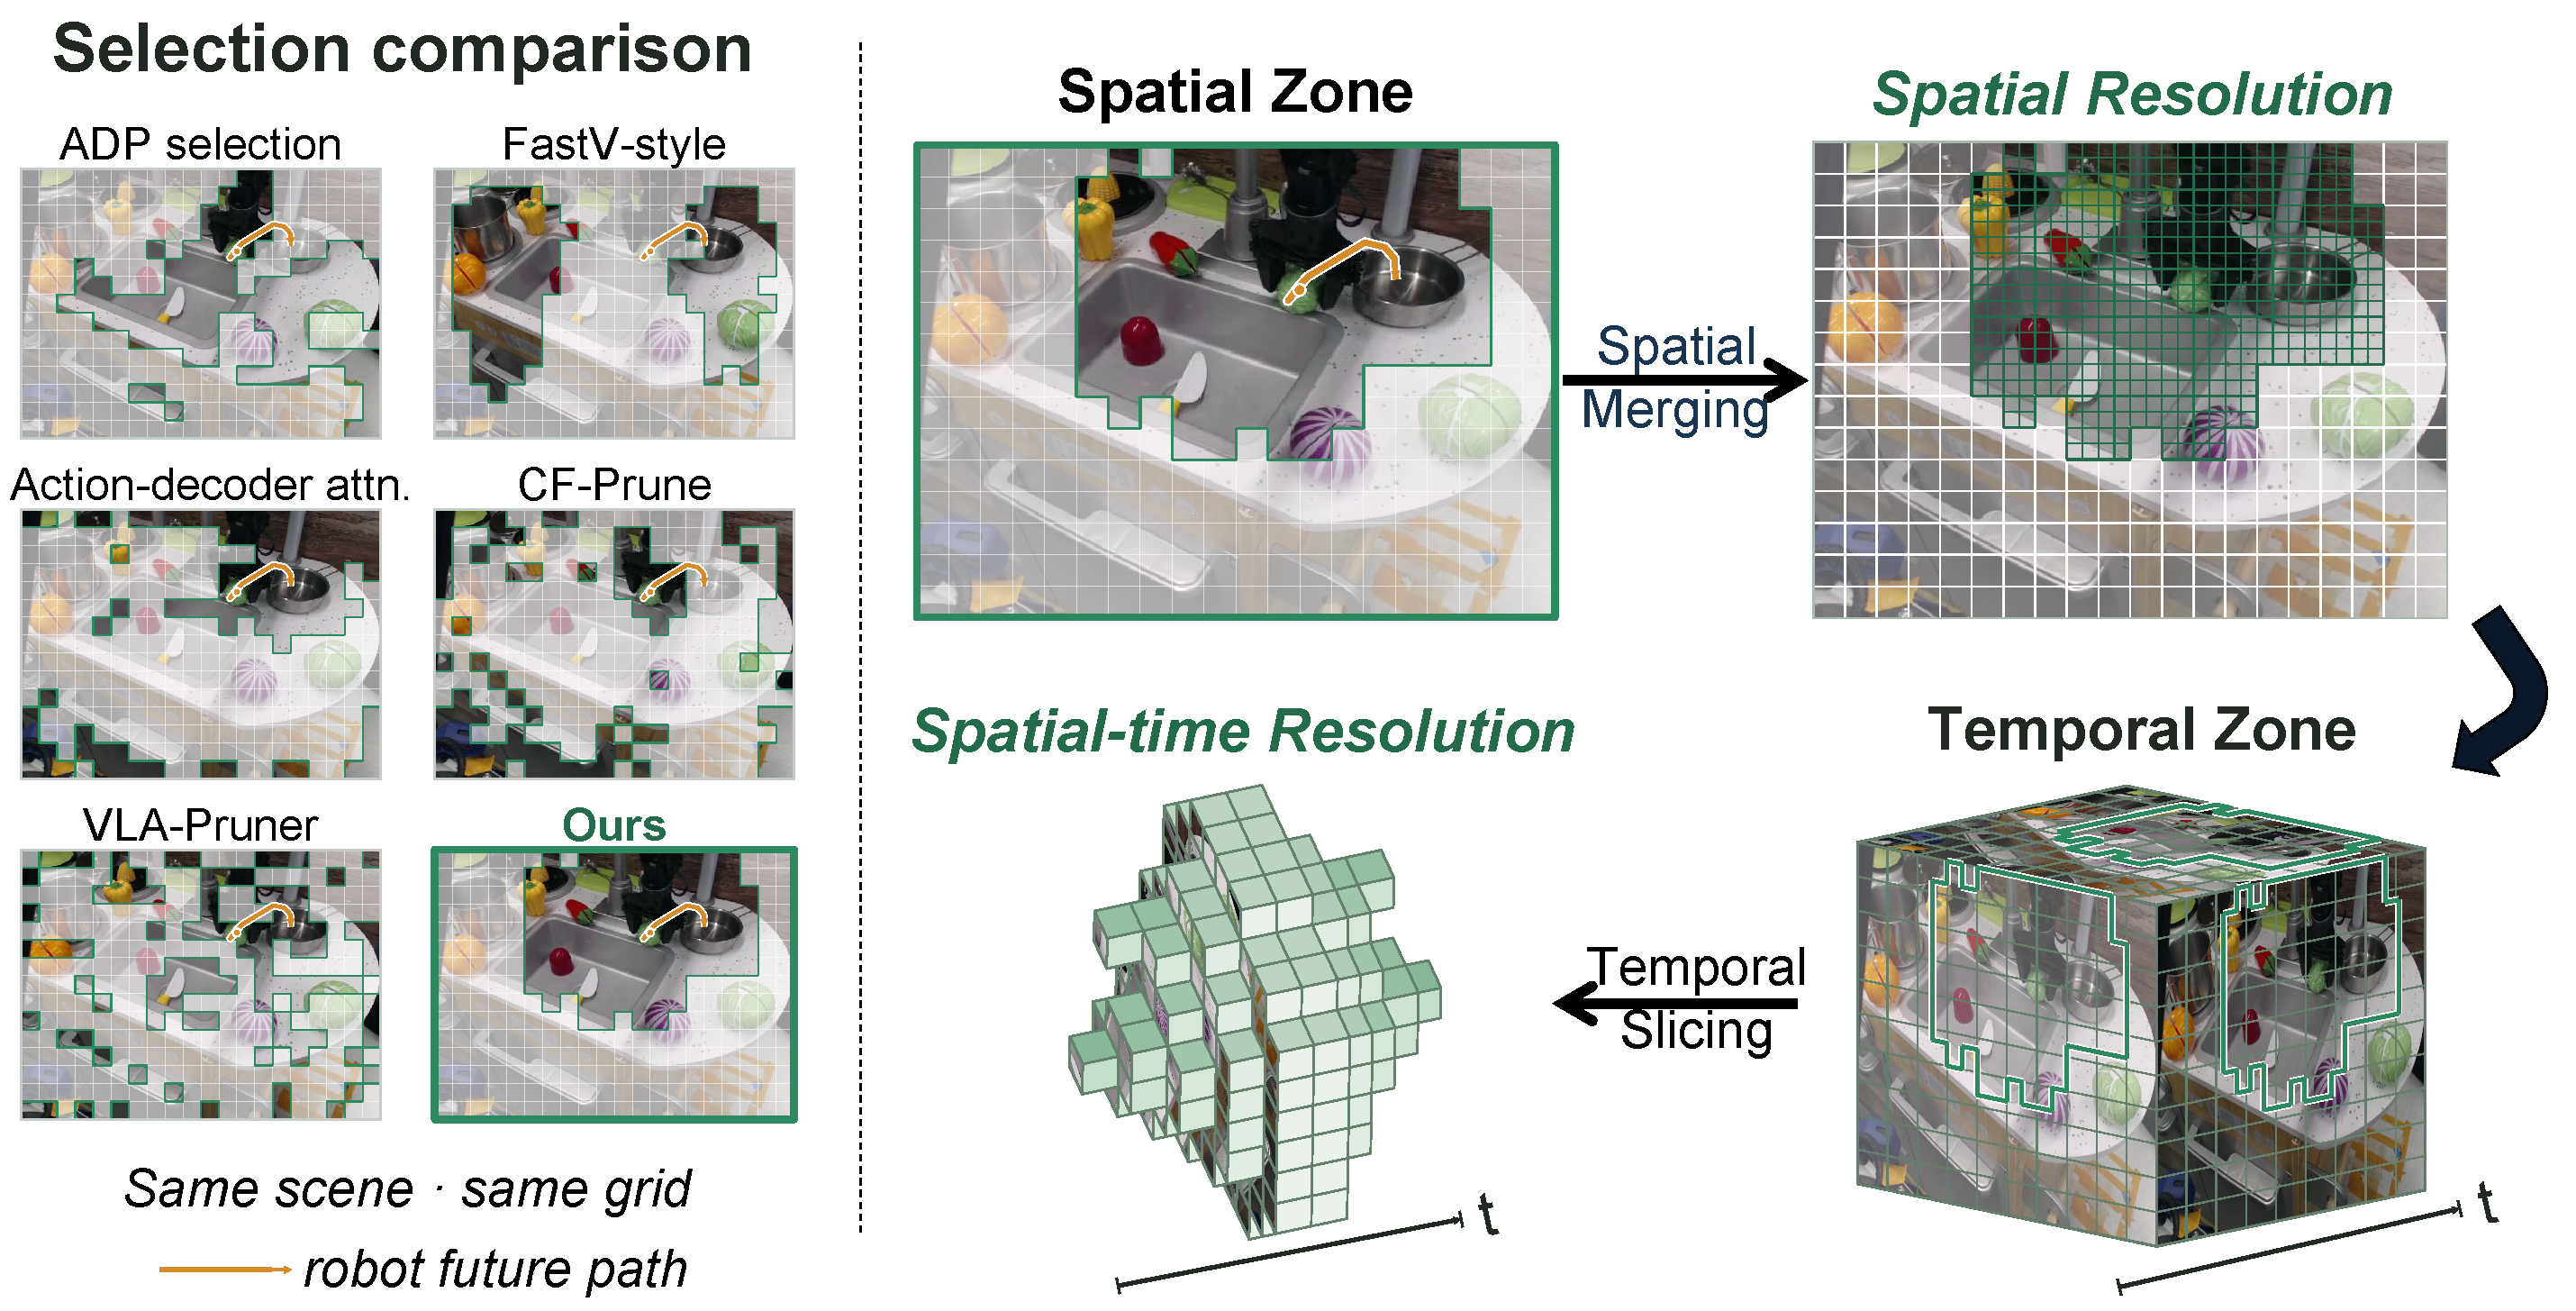
\includegraphics[width=\columnwidth]{teaser_cropped.pdf}
  \caption{\textbf{Action-aware spatial and temporal resolution allocation.}
  Left: example spatial selections for the same scene and grid.
  Right: \method keeps action-relevant regions at high resolution and merges other regions in space and time.
  The orange curve shows future robot motion for reference.}
  \label{fig:teaser}
\end{figure}


A natural tool for making such a representation more compact is token reduction, which merges tokens that look alike~\cite{bolya2023tome} or discards tokens that receive little attention.
These criteria, however, describe the image rather than the task: they measure whether a token is redundant in appearance or salient to the network, not whether the action depends on it.
What is redundant for describing a scene need not be what is irrelevant for acting in it.
Discarding tokens also removes parts of the scene altogether, even though a policy may still need a coarse view of them.
Relevance to the action therefore cannot simply be read off the visual content.

In a WAM, one component already knows what the action needs: the action decoder.
The most direct readout of its needs is its attention over the predicted future.
Attention comes without any training, reflects the action rather than the appearance of the scene, and shows which regions the decoder reads.
As a basis for deciding where the video model computes, however, it has two limitations.
First, it arrives too late: the decoder attends to features that the video model produces late in its forward pass,
so attention exists only after every token of the future has been computed at full resolution, when the computation it could have guided has already been spent.
Second, attention shows where the decoder looks, which need not coincide with how much its prediction would change if a region were represented more coarsely,
and it is the latter that decides whether a region can be coarsened.
What is needed instead is the decoder's judgment, measured by the effect of coarsening on the predicted action and made available early in the video model.
This suggests reversing the usual direction of information flow:
through its objective, the action decoder can teach the video model where to compute in detail and where a coarser view suffices.

Building on this idea, we propose \method, an action-aware router for WAMs (\cref{fig:overview}).
A lightweight router, placed after an early block of the frozen video model, scores every token of the predicted future by its relevance to the action.
It is supervised only through the action decoder:
its training signal is the gradient of the decoder's objective with respect to the scores, and no term depends on appearance or similarity (\cref{sec:router}).
The scores then set the resolution at which the rest of the video model computes each region.
In space, the most relevant regions keep full resolution, while the others are merged into coarser tokens at their original positions rather than removed (\cref{sec:spatial}).
In time, the frames of each region are grouped into segments, more of them for more relevant regions, and the segments keep consecutive temporal positions, matching the frame order the video model was trained on (\cref{sec:temporal}).
Only the router and a low-rank adapter in the action decoder are trained, and the adapter can be merged into the decoder after training.
Because the video model processes fewer tokens after the router, the allocation also reduces computation.

On the three LIBERO task suites~\cite{liu2023libero}, \method keeps 20\% of the future tokens (30\% of all tokens) while remaining statistically indistinguishable from the policy that reads the full representation.
Further analysis shows that the regions it keeps at full resolution are necessary for the policy and concentrate on the robot and the objects it manipulates.

In summary, our contributions are as follows.
\begin{itemize}
  \item An action-aware router for WAMs, supervised only through the objective of the action decoder, which identifies the parts of the predicted future that the action relies on.
  \item A spatial resolution allocation that keeps the most relevant regions at full resolution and merges the others instead of removing them, keeping every token at its original position.
  \item A temporal resolution allocation that gives each region a number of time segments set by its relevance, with consecutive temporal positions.
\end{itemize}

\section{Related Work}
\label{sec:related}

% ---- 脉络--------------------------------------------------------
% 1. World models / 视频生成用于机器人：视频预测作为规划或表征。简短提一下world model随即谈到WAM

% 2. World action models，简要介绍，随即可以对WAM做一些分类。然后分析出他们的特点？然后介绍我们方法能应用到的那一类WAM（先思考这样写好不好，然后再决定）
%    落点：关注"如何从视频得到动作"，把 backbone 的计算当作与动作无关的固定开销。

% 3. 介绍以前的工作在world model或者其他模型上比较有名的方法。然后引出我们的方法和他们的有什么不一样的地方，我们的focus在哪里，优越性在哪里。例如：之前的：Token reduction--图像/VLM（相似度或注意力驱动的合并与剪枝）、视频（时空合并）、VLA 中的剪枝与缓存。

%    然而我们的依据是动作目标学出的相关性，操作是重新分配分辨率，位置处理针对生成式 backbone。
% 4. 扩散模型加速（步数、特征缓存、合并）：正交，可叠加。
% ---------------------------------------------------------------------------

% ---- 起草说明（Claude 记录）--------------------------------------------------
% 分类与图中四类对应：(a) Traditional -> explicit-future；(b) Observed -> observation-conditioned；
%   (c) Joint/Coupled -> joint（shared transformer / mixture of transformers）；(d) Future-conditioned 不变。
%   按"推理时动作如何读取视频模型"归类；跨类的工作（如 PAD、Cosmos Policy 同时生成未来帧）按其核心设计归入一类。
% 对他人工作只写其论文摘要中声明的机制，不引用他们的加速倍数。
% 本节不引用尚未写的 Sec. 5，也不出现 E2 中与 decoder cross-attention 的比较；DeVA 不在论文中出现。
% 2.3 结构：world model 侧（decision-aware world model、轨迹/flow 预测）-> token reduction（VLA 只保留 5 个）-> 三个共性局限 -> 一句话引出方法。
% 所有条目已在 main.bib 中，标题与作者核对自 arXiv 页面（2026-10-26）。
% ---------------------------------------------------------------------------

\subsection{World Action Models}
\label{sec:related_wam}

Learning to predict how the environment evolves has long served robot control.
World models have been used to train policies in imagination~\cite{ha2018worldmodels,hafner2020dreamer,hafner2023dreamerv3},
to plan by predicting the outcomes of candidate actions~\cite{finn2017foresight,zhou2024dinowm,assran2025vjepa2},
and as interactive simulators and data generators~\cite{yang2024unisim,bruce2024genie,jang2025dreamgen}.
Video generation models trained on web-scale video~\cite{nvidia2025cosmos,wan2025wan} now provide such predictions with strong visual and physical priors,
and WAMs turn them into policies that output robot actions~\cite{ye2026dreamzero,pai2025mimicvideo}.
WAMs thereby complement vision-language-action models (VLAs), which build policies on vision-language models~\cite{brohan2023rt2,kim2024openvla,black2025pi0}.

Existing WAMs differ mainly in how the action is obtained from the video model, which also determines what the video model must compute at inference.
\emph{Explicit-future} WAMs generate the future as images or video and act on it:
actions are inferred from generated frames or subgoal images by an inverse dynamics model or a goal-conditioned policy~\cite{du2023unipi,ko2024avdc,black2024susie,tian2024seer,zhao2025cotvla},
or predicted together with the future frames~\cite{wu2024gr1,cheang2024gr2}.
They pay for generating the future at every decision.
\emph{Observation-conditioned} WAMs use video prediction only as a training signal and act from the current observation at test time~\cite{yuan2026fastwam},
similar to policies trained to anticipate embeddings of future observations~\cite{zheng2025flare}.
\emph{Joint} WAMs denoise video and actions together in one network,
either a single transformer that processes observation, future and action tokens~\cite{guo2024pad,li2025uva,zhu2025uwm,kim2026cosmospolicy,ye2026dreamzero}
or a mixture of transformers whose video and action experts interact through joint attention~\cite{li2026lingbotva,bi2026motus}.
\emph{Future-conditioned} WAMs keep the two apart:
the video model predicts the future, and a separate action module reads the video model's internal representation of this prediction~\cite{hu2025vpp,wen2024vidman,liao2025ge,pai2025mimicvideo,ma2026dit4dit}.
The categories overlap, since some joint models also generate future frames and their action tokens attend to future tokens as well;
what separates joint from future-conditioned WAMs is whether video and action are computed in one network or in a cascade.

\subsection{Future-Conditioned World Action Models}
\label{sec:related_future}

Among these designs, future-conditioned WAMs separate prediction from control most cleanly.
The video model is usually trained for prediction first, and a comparatively light decoder then learns to read it~\cite{hu2025vpp,liao2025ge,pai2025mimicvideo}, typically from intermediate features rather than from pixels.
VPP conditions an implicit inverse dynamics model on the future representation inside a video diffusion model~\cite{hu2025vpp},
VidMan turns a video diffusion model pretrained on robot videos into an inverse dynamics model through a layer-wise adapter~\cite{wen2024vidman},
mimic-video cross-attends to an intermediate layer and finds that a single forward pass, without denoising the future frames, already gives strong performance~\cite{pai2025mimicvideo},
and DiT4DiT conditions an action transformer on the features of a video transformer trained together with it~\cite{ma2026dit4dit}.
Because the decoder reads the predicted future through a path of its own, this family is where one can ask most directly which parts of that future the action needs, and it is the setting of this work.
Much of the cost of WAMs lies in the video model, and existing work reduces it by shortening the generation process:
by running fewer denoising steps, down to a single forward pass~\cite{pai2025mimicvideo},
by building the future representation in one pass with learned anticipation tokens instead of an iterative rollout~\cite{zhang2026rift},
or by not predicting the future at test time at all~\cite{yuan2026fastwam}.
General accelerations of diffusion models, through feature caching~\cite{zhao2025pab,liu2025teacache}, sparse attention~\cite{xi2025sparsevideogen}, token merging~\cite{bolya2023tomesd,li2024vidtome} or region-adaptive sampling~\cite{liu2026ras},
aim to preserve the generated images or video, a goal that a policy does not share.
None of these approaches uses the action to decide which parts of the future are computed in detail.


\subsection{Action-Aware Token Selection}
\label{sec:related_tokens}

Deciding which parts of a representation matter for control is a long-standing question for predictive models.
Decision-aware world models learn only what is useful for acting:
value-equivalent models predict just what is needed to plan with values~\cite{grimm2020valueequivalence,schrittwieser2020muzero},
and several world models separate reward-relevant or controllable content from distractors~\cite{fu2021tia,wang2022denoisedmdp,pan2022isodream}.
Other world models keep their representation compact by tokenizing only what changes between frames~\cite{micheli2024deltairis}.
Policies that learn from video likewise predict compact, action-relevant quantities instead of full frames, such as the tracks of points or the flow of objects~\cite{wen2024atm,bharadhwaj2024track2act,xu2024im2flow2act}.
These approaches build relevance into what the model learns to predict, so they require training a new model or representation.
Token reduction keeps the model and reduces the tokens it processes instead,
by merging similar tokens~\cite{bolya2023tome,bolya2023tomesd,li2024vidtome,hyun2025sttm}, by dropping or compressing tokens that receive little attention~\cite{chen2024fastv,liang2022evit,zhang2025sparsevlm},
or with a small selector trained by the task loss~\cite{rao2021dynamicvit,ryoo2021tokenlearner,raposo2024mod}, as RT-1 does for its image tokens with the action loss~\cite{brohan2023rt1}.
Recent VLA methods select visual tokens by their attention to the instruction~\cite{yang2025efficientvla}, by their change between control steps~\cite{xu2025vlacache},
by text relevance gated on the recent motion of the end effector~\cite{pei2026adp}, by semantic attention combined with the action-decoding attention of recent control steps~\cite{liu2025vlapruner}, or with a selector learned while the policy is fine-tuned~\cite{jiang2025lightvla}.
Some training-free methods bring selection to the future tokens of WAMs: they score tokens by action attention~\cite{xie2026sparsewam} or by action and instruction attention~\cite{kim2026cfprune} at the first denoising step and compute only the selected tokens in the remaining steps.

Recent VLA methods select visual tokens by their attention to the instruction~\cite{yang2025efficientvla}, by their change between control steps~\cite{xu2025vlacache},
by the recent motion of the end effector~\cite{pei2026adp}, by the attention of the action-decoding stage~\cite{liu2025vlapruner}, or with a selector learned while the whole policy is fine-tuned~\cite{jiang2025lightvla}.

These methods leave three gaps for our setting.
Relevance is built into a newly trained model, approximated by appearance, attention or motion, or learned by retraining the model whose tokens are selected.
Selection methods usually remove the remaining tokens from the computation, so the corresponding parts of the scene no longer reach the action, while merging methods keep the scene but choose what to merge by visual similarity alone.
In robot policies, selection has mostly acted on the current observation, and the methods that select future tokens need a full-resolution first step and save computation only in later denoising steps, which a video model run for a single forward pass~\cite{pai2025mimicvideo} does not have.
Our router addresses all three:
it is trained only through the objective of the action decoder, leaves the pretrained video model unchanged,
and, from an early block of the video model, gives the regions of the predicted future that the action relies on least a coarser resolution instead of removing them.

\section{Method}
\label{sec:method}

% ---- 草稿说明（改完删除）----------------------------------------------------
% Claude 起草的粗稿，供修改。目前只有 4.1--4.3，不引用尚未写的 Sec. 3 / Sec. 5。
% 所有设置取自已采用格（contiguous-t，2x2 分组、前 100 组满分辨率）。
% 待核对：router 结构与伪标签配方来自已有 KnowledgeRouter 实现，若出自已发表工作需引用。
% ---------------------------------------------------------------------------

\begin{figure*}[t]
  \centering
  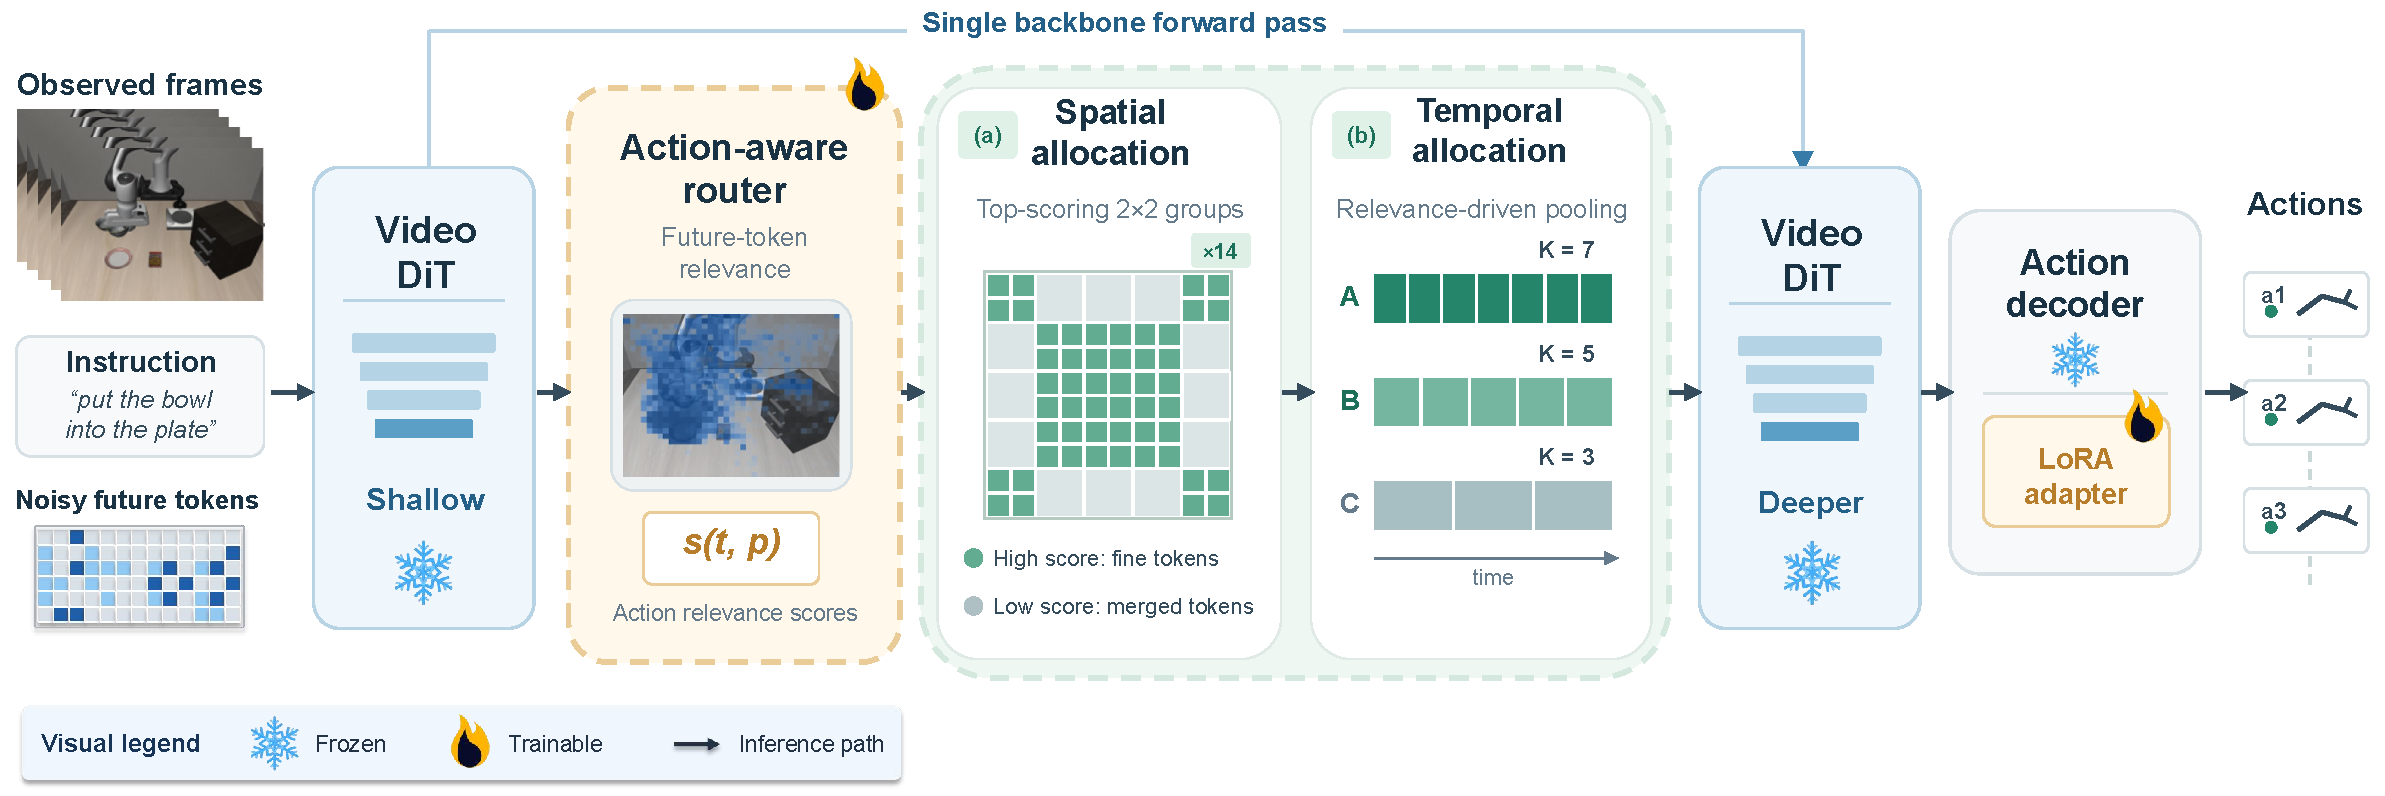
\includegraphics[width=\linewidth]{pipelinev2}
  \caption{\textbf{Overview of \method.}
  After an early block of the frozen video DiT, an action-aware router scores the future tokens.
  Spatially, the highest-scoring $2{\times}2$ blocks keep full resolution and every other block is merged into a single tube;
  temporally, each tube is pooled into a number of segments set by its relevance, and the segments are re-indexed contiguously in time.
  The remaining blocks run on the compact sequence, whose output conditions the action decoder. \cj{XX I'd take out (a) and (b) as a separate figure for each subsection XX}
}
  \label{fig:overview}
\end{figure*}

Our method aims at identifying action-relevant tokens throughout within future representation, which then merge the other tokens to eliminate its negative influences towards both action generation and inference time. Specifically, our method decide the spatial and temporal resolution the backbone computes per region of the scene, using relevance learned from the action decoder.
\cj{XX write Coarse-to-fine ! XX the readers should be able to understand our work from coarse to fine. E.g. formulate the problem and give motivation first as Section 3.1. and then dive into details  }
% ---------------------------------------------------------------------------
\subsection{Action-Aware Router}
\label{sec:router}

The router gives every future token a score between 0 and 1 that indicates how relevant the token is to the action.
It reads the future-frame tokens after the second block of the video DiT together with the instruction:
each token attends to the instruction tokens through one cross-attention layer, and an MLP with a sigmoid outputs its score $s_{t,p}$,
where $t$ indexes the future frame and $p$ the position on the token grid.
The scores provided by this small router then drive both allocation steps (\cref{sec:spatial,sec:temporal}).

The router is trained on the demonstrations of the target task suite, the same data used to train the policy.
Video features are computed as at inference, with the future frames at the inference noise level and the compression applied,
so the router learns on the inputs it will see when deployed.
The video model and the action decoder are frozen.
The router is trained together with a LoRA adapter~\cite{hu2022lora} on the cross-attention layers of the action decoder, which lets the decoder adjust to the compressed input.

The action decoder is a flow-matching model~\cite{lipman2023flow} that predicts a velocity for a noised action chunk.
The adapter is trained on the compressed context to match the output of the same decoder evaluated on the full context, with a small ground-truth term:
\begin{equation}
  \mathcal{L}_{\text{task}} =
  \underbrace{\norm{v - v_{\text{full}}}^2}_{\mathcal{L}_{\text{distill}}}
  + \, 0.02 \underbrace{\norm{v - v_{\text{gt}}}^2}_{\mathcal{L}_{\text{GT}}} ,
  \label{eq:task_loss}
\end{equation}
where $v$ is the velocity predicted by the adapted decoder from the compressed context,
$v_{\text{full}}$ is the velocity predicted by the original decoder from the full context for the same noised action and robot state,
and $v_{\text{gt}}$ is the ground-truth velocity.
$\mathcal{L}_{\text{distill}}$ makes the adapted decoder reproduce the original decoder's full-context prediction, and $\mathcal{L}_{\text{GT}}$ weakly anchors it to the demonstrated ground-truth velocity. Since the adapter only compresses the context rather than learning a new policy, $\mathcal{L}_{\text{distill}}$ is the main objective. This keeps the decoder close to the original policy, so the router signal from $\mathcal{L}_{\text{task}}$ reflects the policy's needs rather than compensating for a drifting decoder; $\mathcal{L}_{\text{GT}}$ only prevents it from drifting too far from the demonstrations.




The adapter only needs to let the decoder read the compressed context, not to learn a new policy.
Distillation keeps the decoder close to the original policy, so the router signal derived from $\mathcal{L}_{\text{task}}$ below reflects what this policy needs, rather than what helps a changing decoder refit the demonstrations;
the ground-truth term only anchors the decoder to the demonstrations.

The router learns which groups of tokens (\cref{sec:spatial}) should keep full resolution under a fixed token budget.
Its supervision is the gradient saliency of the decoder objective with respect to the group scores:
\begin{equation}
  r_g = \max\Big(0,\, -\frac{\partial \mathcal{L}_{\text{task}}}{\partial S_g}\Big),
  \label{eq:saliency}
\end{equation}
where $S_g$ is the score of group $g$ (\cref{eq:group_score}) and $r_g$ measures how much raising it would lower $\mathcal{L}_{\text{task}}$.
Keeping a group at full resolution is a discrete choice, so we multiply its tokens by a straight-through factor~\cite{bengio2013estimating} that equals one in the forward pass; this makes the gradient defined without changing the forward computation.
We smooth $r_g$ with an exponential moving average over training steps, label the top-$k$ groups as relevant and the rest as irrelevant, where $k$ is the number of groups kept at full resolution, and train the router on these labels with
\begin{equation}
  \mathcal{L}_{\text{router}} = \mathcal{L}_{\text{focal}} + \lambda_b \mathcal{L}_{\text{budget}} + \lambda_e \mathcal{L}_{\text{entropy}} ,
  \label{eq:router_loss}
\end{equation}
where $\mathcal{L}_{\text{focal}}$ is a focal binary cross-entropy~\cite{lin2017focal} between the scores and the labels,
$\mathcal{L}_{\text{budget}}$ keeps the mean score at the fraction of groups kept at full resolution,
$\mathcal{L}_{\text{entropy}}$ pushes the scores towards 0 or 1, and $\lambda_b = \lambda_e = 0.1$.


% ---------------------------------------------------------------------------
\subsection{Spatial Resolution Allocation}
\label{sec:spatial}

The video model represents each future frame as a $30{\times}40$ grid of tokens.
We call the sequence of tokens at grid position $p$ across the 14 future frames \emph{tube} $p$, which gives 1,200 tubes.
We then group the tubes into $2{\times}2$ neighborhoods, giving 300 groups.
We use $2{\times}2$ groups for three reasons.
Neighboring tokens cover adjacent image regions, so averaging a small neighborhood still keeps a coarse view of that region.
A $2{\times}2$ group is the smallest square neighborhood, so merging reduces resolution equally in both directions.
And it tiles the $30{\times}40$ grid exactly, so every token belongs to exactly one group.

Each group receives one score from the router:
\begin{equation}
  S_g = \frac{1}{4} \sum_{p \in g} \max_t \, s_{t,p} ,
  \label{eq:group_score}
\end{equation}
where $g$ is a group, $p$ runs over its four positions, and $s_{t,p}$ is the router score of \cref{sec:router}.
Taking the maximum over the future frames means that a position counts as relevant if it matters in any frame;
averaging over the group gives its overall relevance.
During training, the router supervision of \cref{sec:router} is computed on these group scores.

We rank the groups by $S_g$.
The 100 highest-scoring groups keep their four tubes at full resolution.
In every other group, the four tubes are averaged frame by frame into a single tube.
This leaves 600 tubes, and no region of the scene is removed: relevant regions keep full resolution and the rest are kept at a coarser one.
The group scores thus decide which regions of the scene the backbone sees in detail, and the number of full-resolution groups sets how many.

Every tube keeps its position on the original grid; a merged tube takes the position $p$ of the top-left tube of its group,
so every remaining tube is still identified by a grid position $p$.
We do not re-index the tubes onto a smaller grid:
the observation frames stay on the original grid, so a future tube at position $p$ still refers to the same part of the scene as the observed tokens at $p$.

% ---------------------------------------------------------------------------
\subsection{Temporal Resolution Allocation}
\label{sec:temporal}
% 按现行实现写：排序用组分数 x 帧间特征变化，切点使各段覆盖的特征变化相近。按约定不写"按运动自适应"、不声称优于固定 K。
% 诊断事实：段数档位与满分辨率/合并划分完全重合，给定段数时切点近乎均匀，部署时不同观测间段数分配 97.3% 相同。

Since the scene is changing as the robot and the objects move, the action-relevant content of a region also changes over the prediction horizon.
Regions that matter for the action therefore need finer temporal detail to follow how they evolve, while other regions are adequately described by a few tokens.
We therefore give each tube its own temporal resolution as a single temporal resolution shared by all tubes cannot reflect this. So we further split 14 frames into a few consecutive segments, where the tokens within each segment are averaged into one.
Tubes are split into $K$ segments, and more segments mean finer temporal detail.

The number of segments follows relevance.
Each tube $p$ receives a priority
\begin{equation}
  u_p = S_{g(p)} \cdot \Delta_p ,
  \label{eq:priority}
\end{equation}
where $S_{g(p)}$ is the score (\cref{eq:group_score}) of the group $g(p)$ that contains position $p$,
and $\Delta_p$ is the average change of the features of tube $p$ between consecutive frames, measured as one minus their cosine similarity.
A tube thus ranks high when it is relevant to the action and its features change across frames.
We give the most segments to the tubes with the highest priority, with a fixed number of tubes at each level.
For example, when 10\% of the future tokens are kept, the top 300 tubes receive 4 segments, the next 180 receive 2, and the last 120 receive 1, giving 1,680 tokens.
Within a tube, segment boundaries are placed so that each segment covers a similar amount of feature change.

As a result, temporal detail is concentrated on the tubes that matter for the action.
Every tube keeps at least one token, so no region disappears from the sequence, and averaging rather than dropping frames keeps information from all of them.
Because the number of tubes at each level is fixed, every sample is represented by the same number of tokens, independent of the scene.

\begin{figure}[t]
  \centering
  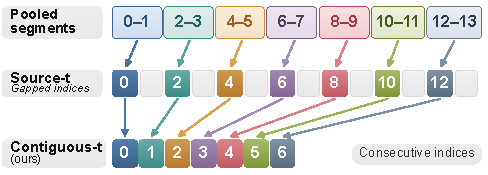
\includegraphics[width=\linewidth]{contiguous_t.pdf}
  \caption{\textbf{Temporal positions after segment pooling.}
  The same four segments are assigned representative source-frame positions $(1,4,8,11)$ by source-t, or consecutive positions $(0,1,2,3)$ by contiguous-t.
  Positions are relative to the future sequence in this illustration; the pooled segment features are the same before position encoding.}
  \label{fig:temporal_positions}
\end{figure}

The $k$-th segment of every tube takes the $k$-th future time position, whichever frames it covers, so the temporal positions stay consecutive as in the original sequence.
\Cref{fig:temporal_positions} illustrates these indices alongside the source-t alternative for the same pooled segments.
This differs from the spatial axis (\cref{sec:spatial}) because the two kinds of position carry different information.
A spatial position says where a token lies in the scene, and it must stay aligned with the observation frames, which remain on the original grid.
A temporal position only says in which order the future frames come.
After slicing, a segment spans several frames, so no single original frame index describes it; what must be preserved is the order of the segments.
Consecutive indices keep this order and match the pattern of consecutive frames the video model was trained on,
whereas original frame indices would leave gaps between segments, a pattern the model never sees during training.
% 实验依据（写 Sec. 5 时用，正文暂不引用）：
%   空间：2x1 池化后改为紧凑重编号 4/100 vs 保留原坐标 83/100（LIBERO-Spatial 7200 tok，n=100）。
%   时间：contiguous vs source 354 vs 275、441 vs 396、460 vs 437（10/20/30%，n=500，配对 McNemar 均 p<0.005）。
%   "时间位置是槽位"是解释，只能写"一致于"，不能写"证明"。

\section{Experiments}
\label{sec:exp}

% ---- 脉络）--------------------------------------------------------
% 0. Setup：LIBERO 套件；n=500 逐 episode 配对；exact McNemar；预算定义
%    （keep ratio 只作用于 future token，obs token 全保留——务必写清楚）。
% 1. 主结果：成功率--token 预算曲线；对照 native、LoRA 匹配的全上下文、
%    同 router 的 token/tube 删除。对 native 只写"不可区分"。
% 2. 效率：FLOPs、video DiT 延迟、端到端延迟（含固定开销；分别报有无 CUDA graphs）。
%    另含：router + 分配链的开销；LoRA fold 前后的闭环对比与延迟；
%    各预算的 K 档与配额表（Method 4.3 用 \cref{sec:exp} 指向这里）。
% 3. 消融（每个组件一组）：router 训练方式；合并 vs 删除；时间位置 contiguous vs source；
%    空间位置；有无 adapter。
% 4. 泛化：其他套件、LIBERO-Plus、第二个 backbone。
% 5. 分析：router 选择的可视化；激进预算下失败集中的任务。
% 表格放在 tables/ 下，用 \input{tables/<name>} 引入；label 用 tab:<name>。
% ---------------------------------------------------------------------------

\subsection{Experimental Setup}
\label{sec:exp_setup}

We evaluate \method on LIBERO-Spatial, LIBERO-Object and LIBERO-Goal~\cite{liu2023libero}, using the released suite-specific mimic-video checkpoints~\cite{pai2025mimicvideo}.
Each suite contains ten tasks; we run 50 episodes per task and report the success rate over 500 episodes.
Within each suite, all configurations use evaluation seed 0 and the same initial states, allowing outcomes to be paired episode by episode.
The video model runs a single forward pass, and the policy executes five predicted actions before replanning.
Our reference is the native policy: the original video model and action decoder evaluated on the full token sequence.

The budget is the fraction of the 16,800 future tokens retained after the second video DiT block; all 2,400 observation tokens remain.
Keeping 10\%, 20\% and 30\% of the future tokens gives sequences of 4,080, 5,760 and 7,440 tokens, respectively, compared with 19,200 for native.
The spatial allocation keeps 100 of the 300 groups at full resolution at every budget.
In order of increasing priority, the three temporal tiers contain 120, 180 and 300 tubes; their segment counts are $(1,2,4)$, $(3,5,7)$ and $(5,8,10)$ at the three budgets, respectively.

For each suite, we freeze a router trained on that suite and train a fresh rank-16 low-rank adapter (LoRA) in the decoder cross-attention for each budget.
The video model and the original decoder weights remain frozen.
Each adapter is trained for 1,500 steps with the objective in \cref{eq:task_loss}, a learning rate of $4\times10^{-5}$, 100 warmup steps, cosine decay and an effective batch size of eight.
The Object router uses a different initialization and training recipe: fixed segment counts of $8/6/4$ and pure distillation, whereas the Spatial and Goal routers use $12/10/8$ and the additional ground-truth term of weight 0.02.
This difference concerns router training; the budget-specific adapters use the same objective on all three suites.
We use one training seed per configuration.

We compare paired success outcomes with two-sided exact McNemar tests and apply Holm correction over the nine suite--budget comparisons with native, at a significance level of 0.05.
The error bars and native bands in \cref{fig:main_results} are Wilson 95\% confidence intervals for the individual success rates.
Non-significant comparisons are described as statistically indistinguishable at this sample size.

\subsection{Main Results}
\label{sec:exp_main}

\begin{figure*}[t]
  \centering
  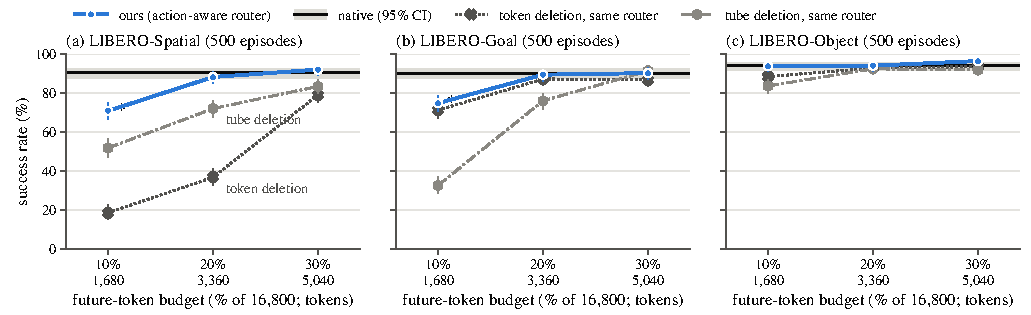
\includegraphics[width=\linewidth]{fig4_main_results.pdf}
  \caption{\textbf{Success rate versus future-token budget.}
  Each point uses 500 paired episodes; the 2,400 observation tokens are always kept.
  Blue: \method; black line and grey band: native, which reads all 16,800 future tokens.
  Grey curves (Spatial only): token or tube deletion using the same router and the same budgets, each with its own trained low-rank adapter.
  Token deletion keeps the highest-scoring future tokens; tube deletion keeps the highest-scoring tubes with all 14 frames.
  Error bars and band: Wilson 95\% confidence intervals.
  Asterisks mark \method results that differ from native under two-sided exact McNemar tests with Holm correction over the nine suite--budget comparisons.
  The Object router uses the distinct training recipe described in \cref{sec:exp_setup}.}
  \label{fig:main_results}
\end{figure*}

At 20\% of the future tokens, \method is statistically indistinguishable from native on all three suites (\cref{fig:main_results}).
Success rates are 88.2\% on Spatial, 94.0\% on Object and 89.4\% on Goal, compared with 90.4\%, 94.0\% and 90.2\% for native.
The corresponding uncorrected paired-test $p$-values are 0.22, 1.00 and 0.71; none is significant after correction.
At this operating point, the remaining video blocks and action decoder receive 5,760 tokens, or 30\% of the native sequence.

The effect of a tighter budget differs across suites.
At 10\% of the future tokens, success falls to 70.8\% on Spatial and 74.8\% on Goal, both significantly below native after correction, while Object reaches 93.8\% and remains statistically indistinguishable from native.
At 30\%, the respective success rates on Spatial, Object and Goal are 92.0\%, 96.4\% and 90.2\%; all three are statistically indistinguishable from native after correction.
Thus, 20\% of the future tokens is the smallest tested budget at which all three suites are statistically indistinguishable from native in this evaluation.

\TODO{Remaining experiments: merging versus deletion; contiguous versus source temporal positions; E1--E3 action-relevance analyses; transfer to DiT4DiT if included.}
\TODO{Efficiency: FLOPs and latency of the deployed contiguous-t budgets have not been measured.}

\section{Conclusion}
\label{sec:conclusion}

% ---- 脉络（写完删除）--------------------------------------------------------
% 一段：重申"生成形状 vs 控制形状"的论点 -> 三个组件 -> 主结果 -> 对 WAM 设计的启示。
% Limitations（可并入本节或单独成段）：
%   - 结论依赖运行点（future 帧近似噪声占位是 tau_v = 1 时的事实）；
%   - 分配在套件内相对稳定，价值在"放在哪里"而非"逐步追踪场景"；
%   - 蒸馏目标的最优解即 teacher，"不可区分"是该目标下的上限；
%   - 时间轴仍有空间（真实未来运动 oracle 离线更优，但推理时不可得）；
%   - 主要在单一 backbone 上验证。
% ---------------------------------------------------------------------------

\TODO{Conclusion and limitations.}


% The base model is cited in any case; \nocite keeps BibTeX from failing while
% the text has no \cite yet. Harmless to keep.
\nocite{pai2025mimicvideo}
{
    \small
    \bibliographystyle{ieeenat_fullname}
    \bibliography{main}
}

%%%%%%%%% SUPPLEMENTARY
% \suppltrue appends the supplementary to this PDF (e.g. for arXiv or for
% splitting off later). For the CVPR submission keep \supplfalse and upload
% the supplementary as a separate PDF.
\newif\ifsuppl
\supplfalse
\ifsuppl
  \clearpage
\setcounter{page}{1}
\maketitlesupplementary

\setcounter{section}{0}
\renewcommand{\thesection}{\Alph{section}}
\renewcommand{\theHsection}{supp.\arabic{section}}
\setcounter{table}{0}
\renewcommand{\thetable}{S\arabic{table}}
\renewcommand{\theHtable}{supp.\arabic{table}}
\setcounter{figure}{0}
\renewcommand{\thefigure}{S\arabic{figure}}
\renewcommand{\theHfigure}{supp.\arabic{figure}}

% Compiled only when main.tex sets \suppltrue.
% Sections here can be referenced from the main paper (e.g. \cref{sec:supp_impl}) and vice versa.

% ---- 可能的内容（写完删除）--------------------------------------------------
% 实现细节与超参数；统计协议（配对方式、McNemar、CI）；逐任务完整结果；
% 额外的分析与可视化；运行时间测量方式；失败案例；视频说明。
% ---------------------------------------------------------------------------

\section{Implementation Details}
\label{sec:supp_impl}

The main text specifies the LIBERO training and evaluation settings.
The Object router uses pure distillation during router training, while all budget-specific decoder adapters use distillation plus the 0.02-weight ground-truth term.
Bridge uses its separately trained pure-distillation router; its training data and camera setup differ from LIBERO.
For DiT4DiT, the 442-token LIBERO setting pools all future spatial groups and additionally coarsens the observed slice; it is not the 589-token future allocation with only the observation budget changed.

\section{Statistical and Efficiency Details}
\label{sec:supp_stats}

% Paired comparisons of ARROW on mimic-video: against native (left) and against the full-context LoRA control (right).
% 2026-11-11: the two former tables (ours vs native; mimic-video rows of ours vs native + LoRA) were merged here.
% The DiT4DiT differences of the former second table are given in the text of the supplement.
\begin{table*}[t]
  \centering
  \caption{\textbf{Paired comparisons of \method on mimic-video.}
  Every cell has 500 paired episodes.
  $\Delta$ is \method minus the reference in percentage points, with unadjusted paired Wald 95\% intervals.
  $p_H$ is Holm-corrected; each reference forms its own family of nine tests.
  The nominal Object 30\% intervals do not establish significance after correction.}
  \label{tab:paired_uncertainty}
  \small
  \setlength{\tabcolsep}{6pt}
  \begin{tabular}{lr lr lr}
    \toprule
    & & \multicolumn{2}{c}{vs.\ native} & \multicolumn{2}{c}{vs.\ native + LoRA} \\
    \cmidrule(lr){3-4} \cmidrule(lr){5-6}
    Suite & Future & $\Delta$ [95\% CI] & $p_H$ & $\Delta$ [95\% CI] & $p_H$ \\
    \midrule
    Spatial & 10\% & $-19.6$ [$-24.0$, $-15.2$] & $4.8\!\times\!10^{-16}$ & $-20.8$ [$-25.0$, $-16.6$] & $1.4\!\times\!10^{-19}$ \\
    Spatial & 20\% & $-2.2$ [$-5.4$, $+1.0$] & 1.00 & $-3.4$ [$-6.4$, $-0.4$] & 0.24 \\
    Spatial & 30\% & $+1.6$ [$-1.2$, $+4.4$] & 1.00 & $+0.4$ [$-2.4$, $+3.2$] & 1.00 \\
    \addlinespace[2pt]
    Object & 10\% & $-0.2$ [$-2.8$, $+2.4$] & 1.00 & $+0.6$ [$-2.1$, $+3.3$] & 1.00 \\
    Object & 20\% & $+0.0$ [$-2.3$, $+2.3$] & 1.00 & $+0.8$ [$-1.6$, $+3.2$] & 1.00 \\
    Object & 30\% & $+2.4$ [$+0.3$, $+4.5$] & 0.25 & $+3.2$ [$+0.9$, $+5.5$] & 0.063 \\
    \addlinespace[2pt]
    Goal & 10\% & $-15.4$ [$-19.6$, $-11.2$] & $1.6\!\times\!10^{-11}$ & $-15.0$ [$-19.3$, $-10.7$] & $2.2\!\times\!10^{-10}$ \\
    Goal & 20\% & $-0.8$ [$-4.0$, $+2.4$] & 1.00 & $-0.4$ [$-3.6$, $+2.8$] & 1.00 \\
    Goal & 30\% & $+0.0$ [$-2.9$, $+2.9$] & 1.00 & $+0.4$ [$-2.5$, $+3.3$] & 1.00 \\
    \bottomrule
  \end{tabular}
\end{table*}


Confidence intervals describe paired episode differences, not variation over independently trained models.
All adapter configurations use one training seed.
The nine mimic-video ours--native comparisons in the main table use a common Holm family; its Object 30\% adjusted $p$-value is 0.250.
The deletion reference comparisons are separate from that family and do not change the dagger marks.
The original Goal/Object ours--deletion analysis uses a post-hoc family of 12 contrasts, as documented with the results.

The timing benchmark uses Spatial checkpoints on an exclusively allocated H100, batch size one, with text encoding included.
There are three warmup calls and eight interleaved rounds of four calls per arm; reported values are medians of 32 synchronized wall-clock measurements.
The graphed native reference is 701.7\,ms; the eager native reference has median 770.4\,ms across the three budget runs.
The deployed 10\%/20\%/30\% configurations run in 404.2/440.7/477.1\,ms and use 35.7/42.7/49.6 TFLOPs per query.
Speedups relative to graphed native are reported in the main text; relative to the pooled eager reference they are approximately $1.91\times$, $1.75\times$ and $1.61\times$.
The folded-adapter configuration is the one used for timing; these measurements are not a separate closed-loop evaluation of graph/fold equivalence.
For DiT4DiT, an exclusively allocated H100 runs ten warmup calls and 50 measured calls per configuration, with batch size one and no CUDA graphs.
The synchronized wall-clock measurement includes the single-frame VAE and uses cached text; native and compressed configurations share both conventions and stop at the action head's extraction layer.
Native takes 57.7\,ms; the evaluated 589/442/391-token configurations with unfused LoRA take 66.2/66.6/66.9\,ms.
Separate stage measurements show backbone time of 21.7\,ms for native versus 24.2--24.5\,ms compressed, and action-head time of 22.1\,ms versus 28.6--28.7\,ms with LoRA.
These measurements establish overhead at these stages, but do not isolate a kernel-level cause.
Disabling the LoRA branch gives a 60.2--60.9\,ms compute proxy; a policy with folded trained weights has not been validated, so this proxy is not substituted for the evaluated latency.

The earlier DiT4DiT FLOPs comparison uses a released 4.91-TFLOP pipeline with a padded VAE encode.
Encoding only the real observed frame reduces this to 2.90 TFLOPs and is shared by native and ours.
With this common change, the evaluated 589/442/391-token configurations use 2.45/2.10/1.98 TFLOPs including VAE; the main table excludes the common 0.67-TFLOP VAE cost.
Thus the earlier reductions relative to the released path describe arithmetic, not wall-clock speedup or compression alone.
\TODO{Numerical equivalence checks for the deployed mimic-video fold/graph configuration and deletion/external-method timing.}

\section{Original External-Policy Adaptations}
\label{sec:supp_original_external}

% Source: main_results_dit4dit_sources.json; original 2026-11-05 protocol.
\begin{table*}[t]
  \centering
  \caption{\textbf{Original external-policy adaptations on DiT4DiT.}
  These results retain the initial observation-preserving selectors, VLA-Pruner's three dense warm-start queries and ADP's trajectory-gated dense fallback.
  Target is the compressed-branch length; Mean is the per-episode mean context averaged across all three suites, including dense calls.
  Each completed success rate uses 500 paired episodes.
  CF-sel.'s additional full-context probe is extra work beyond the retained context; no-LoRA is the training-free selection arm.
  These are distinct from the fixed-budget selection ports described in this section.}
  \label{tab:dit4dit_original_external}
  \footnotesize
  \setlength{\tabcolsep}{5pt}
  \begin{tabular}{lrrrrrr}
    \toprule
    Original adaptation & Target & Mean context & Spatial & Object & Goal & Avg. \\
    \midrule
    FastV-style & 589 & 589.0 & 98.0 & 100.0 & 98.4 & 98.8 \\
    VLA-Pruner & 589 & 630.9 & 98.6 & 99.6 & 98.8 & 99.0 \\
    ADP & 589 & 703.4 & 98.0 & 99.8 & 97.6 & 98.5 \\
    CF-sel. + LoRA & 589 & \TODO{--} & 98.8 & \TODO{--} & 98.6 & \TODO{--} \\
    CF-sel., no LoRA & 589 & 589.0 & 98.4 & 100.0 & 98.4 & 98.9 \\
    \midrule
    FastV-style & 442 & 442.0 & 94.4 & 99.4 & 92.4 & 95.4 \\
    VLA-Pruner & 442 & \TODO{--} & 97.4 & \TODO{--} & 97.8 & \TODO{--} \\
    ADP & 442 & 638.5 & 98.4 & 99.6 & 98.4 & 98.8 \\
    CF-sel. + LoRA & 442 & 442.0 & 97.2 & 99.2 & 96.4 & 97.6 \\
    CF-sel., no LoRA & 442 & 442.0 & 96.2 & 97.8 & 93.6 & 95.9 \\
    \bottomrule
  \end{tabular}
\end{table*}


The original VLA-Pruner and ADP adaptations use more context than their compressed-branch targets because of dense calls (\cref{tab:dit4dit_original_external}).
They therefore do not constitute fixed-context comparisons.
The main table instead reserves explicit fixed-budget selection ports (FB), with 392/197, 344/98 and 293/98 observed/future tokens at 589, 442 and 391 total context tokens.
ADP-sel. removes trajectory-gated dense fallback and tests the text-guided selection component.
VLA-sel. uses three semantic-only compressed bootstrap queries and scatters their action attention to source positions before maintaining its causal history.
FastV-style and CF-sel. also select observation tokens at the two lower budgets; their selection scores and source positions remain method-specific.
CF-sel. retains a paid full-context probe, which must be included in its inference cost.
All fixed-context ports use a fresh matched decoder adapter; their old-policy success rates are not reused.

\section{Additional Transfer and Router-Training Results}
\label{sec:supp_transfer}

With 100 full-resolution groups, the three Bridge budgets give 20/96, 24/96 and 27/96 successes, versus 46/96 for native.
Their paired differences are $-27.1$ [$-38.1$,$-16.1$], $-22.9$ [$-32.7$,$-13.1$] and $-19.8$ [$-29.6$,$-9.9$] percentage points, with exact McNemar $p=1.3\times10^{-5}$, $2.7\times10^{-5}$ and $3.1\times10^{-4}$, respectively.
These failed points motivate reporting the entire higher-budget $F=200$ sweep rather than only its best point estimate.

The original $F=200$, 11,400-token run gives 45/96 successes (46.9\%), versus 46/96 for native; its paired difference is $-1.0$ points [95\% CI $-9.9$,$+7.9$], with discordant counts 9/10 and exact McNemar $p=1.00$.
The 50.0\% point estimate in the transfer table comes from a separate run on another machine with a different seed.
Its interval and paired comparison remain pending; the original run's interval is not reused for it.

Earlier combined spatial/temporal DiT4DiT configurations on GR1 have lower point estimates than native.
For example, the future-space/time 441-token configuration with 41 full-resolution groups reaches 53.2\%, versus 54.9\% for native, a $-1.8$ point difference with interval [$-4.5$,$+1.0$].
The completed 466-token follow-up keeps 41 future $2\times2$ groups at full resolution and merges 74 spatial tubes across time; it removes 48 tokens spatially and 74 temporally while leaving the observation unchanged.
Its frozen router and 1,500-step decoder adapter yield 660/1,200 successes, versus 659/1,200 for native.
The paired difference is $+0.08$ points [95\% CI $-2.66$,$+2.83$], with discordant counts 142/141 and exact McNemar $p=1.00$.
This configuration was selected after inspecting the intermediate 441-token results and uses one training seed.
It demonstrates simultaneous spatial and temporal allocation in this evaluated setting, but its confidence interval does not establish equivalence to native.

Continuing to train the router jointly with the adapter for 1,500 steps gives the following success rates, in 10\%/20\%/30\% budget order:
Spatial 72.2/90.8/91.6\%, Goal 76.2/86.2/89.4\%, and Object 91.8/94.4/96.0\%.
Relative to frozen-router training, no improvement survives Holm correction over nine suite--budget comparisons; the pooled, post-hoc paired test has $p=0.83$.
The individual adjusted $p$-values, in the same order, are 1.00/0.68/1.00, 1.00/0.10/1.00 and 0.77/1.00/1.00.
This is a lack of detected benefit for that recipe and sample size, not evidence of equivalence.

\section{Detailed Action-Relevance Analysis}
\label{sec:supp_relevance}

\begin{figure*}[t]
  \centering
  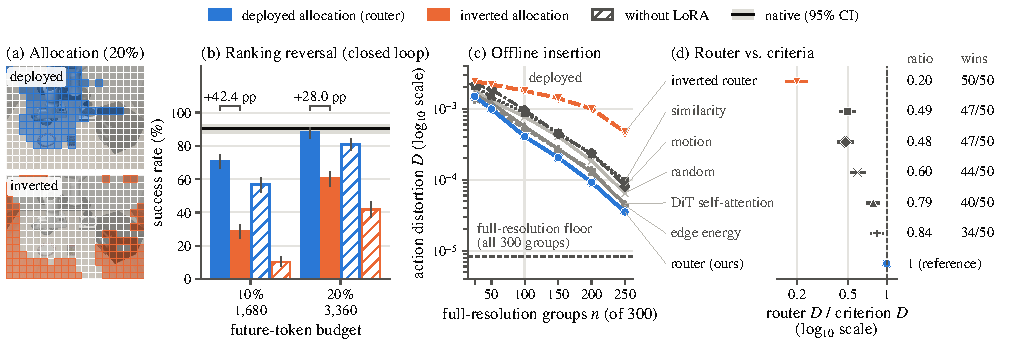
\includegraphics[width=\linewidth]{fig5_action_relevance.pdf}
  \caption{\textbf{Ranking reversal and offline action distortion.}
  (a) Deployed and inverted full-resolution groups at the same budget.
  (b) Spatial success over 500 paired episodes, with separately trained low-rank adapters (solid) or without adapters (hatched); bars show Wilson 95\% confidence intervals.
  (c) Spatial insertion curves over 200 windows from 50 held-out episodes: the top-$n$ groups retain full resolution, the rest are merged, and all 14 future frames remain.
  Distortion is the normalized mean squared difference from the native decoder's first five actions under full context, geometrically averaged over windows.
  The dashed line is the full-resolution numerical floor.
  (d) Router-to-criterion distortion ratios, averaged over six group counts in log space, with episode-level Student's $t$ 95\% intervals.
  The five criteria are similarity, motion, block-2 self-attention, observed-frame edge energy and random selection.}
  \label{fig:supp_relevance}
\end{figure*}

The pre-registered offline family also included full-context decoder cross-attention, which has approximately 7\% lower distortion than the router ($p=0.0078$ after correction).
It requires completing the uncompressed video/decoder forward pass and therefore is not an equal-cost block-2 scoring substitute.
Claims of superiority apply only to the five task-agnostic criteria shown in the figure.
Similarity ranking in this analysis is not a complete ToMe implementation.
The matched offline coverage-versus-resolution comparison does not distinguish the two allocations after correction, so it is not used to attribute the closed-loop operator gap to coarse coverage alone.

\section{Absolute Cross-Policy Success Rates}
\label{sec:supp_absolute}

\begin{table*}[t]
  \centering
  \caption{\textbf{Absolute LIBERO success rates for context.}
  Avg. is recomputed over Spatial/Object/Goal only; LIBERO-Long is omitted for every row.
  Published rows have different training, sensing and evaluation protocols and are not matched compression baselines.
  Source links identify the actual result table or release, including secondary reporting where used.
  Our rows repeat \mainref{tab:main_results}{Table~1}.
  The table also includes SmolVLA and Cosmos Policy, which are omitted from the parameter bubble figure.}
  \label{tab:absolute_success}
  \small
  \setlength{\tabcolsep}{6pt}
  \begin{tabular}{lrrrrl}
    \toprule
    Policy & Spatial & Object & Goal & Avg. & Result source \\
    \midrule
    OpenVLA & 84.7 & 88.4 & 79.2 & 84.1 & \href{https://arxiv.org/abs/2406.09246}{App. E} \\
    OpenVLA-OFT & 97.6 & 98.4 & 97.9 & 98.0 & \href{https://arxiv.org/abs/2502.19645}{Tab. I} \\
    $\pi_0$ & 96.8 & 98.8 & 95.8 & 97.1 & \href{https://arxiv.org/abs/2502.19645}{Tab. I} \\
    $\pi_{0.5}$ & 98.8 & 98.2 & 98.0 & 98.3 & \href{https://huggingface.co/docs/lerobot/libero}{OpenPI results} \\
    $\pi_0$-FAST & 96.4 & 96.8 & 88.6 & 93.9 & \href{https://arxiv.org/abs/2502.19645}{Tab. I} \\
    Octo & 78.9 & 85.7 & 84.6 & 83.1 & \href{https://arxiv.org/abs/2406.09246}{App. E} \\
    SpatialVLA & 88.2 & 89.9 & 78.6 & 85.6 & \href{https://arxiv.org/abs/2501.15830}{Tab. III} \\
    CoT-VLA & 87.5 & 91.6 & 87.6 & 88.9 & \href{https://arxiv.org/abs/2503.22020}{LIBERO results} \\
    UniVLA & 96.5 & 96.8 & 95.6 & 96.3 & \href{https://arxiv.org/abs/2505.06111}{Tab. I} \\
    NORA-Long & 92.2 & 95.4 & 89.4 & 92.3 & \href{https://arxiv.org/abs/2504.19854}{Tab. 2} \\
    VLA-RL & 90.2 & 91.8 & 82.2 & 88.1 & \href{https://arxiv.org/abs/2505.18719}{Tab. 1} \\
    WorldVLA & 87.6 & 96.2 & 83.4 & 89.1 & \href{https://arxiv.org/abs/2506.21539}{Tab. 2} \\
    SmolVLA (0.45B) & 90.0 & 96.0 & 92.0 & 92.7 & \href{https://arxiv.org/html/2506.01844v1}{Tab. 2} \\
    SmolVLA (2.25B) & 93.0 & 94.0 & 91.0 & 92.7 & \href{https://arxiv.org/html/2506.01844v1}{Tab. 2} \\
    Cosmos Policy & 98.1 & 100.0 & 98.2 & 98.8 & \href{https://research.nvidia.com/labs/cosmos-lab/cosmos-policy/}{Author results} \\
    \midrule
    mimic-video native & 90.4 & 94.0 & 90.2 & 91.5 & Our evaluation \\
    mimic-video+ (20\% future) & 88.2 & 94.0 & 89.4 & 90.5 & Our evaluation \\
    DiT4DiT native & 98.6 & 99.4 & 98.6 & 98.9 & Our evaluation \\
    DiT4DiT+ (589 tokens) & 99.2 & 100.0 & 98.6 & 99.3 & Our evaluation \\
    \bottomrule
  \end{tabular}
\end{table*}


The results in \cref{tab:absolute_success} provide context rather than a common-backbone or common-protocol comparison.
The main claims concern changes relative to each policy's own native backbone.
For $\pi_0$ and $\pi_0$-FAST, the listed numbers are the released-model results tabulated by OpenVLA-OFT; $\pi_{0.5}$ uses the OpenPI release numbers reproduced in the LeRobot documentation.
The three-suite means are recomputed, rather than copied from four-suite LIBERO averages.

\begin{figure*}[t]
  \centering
  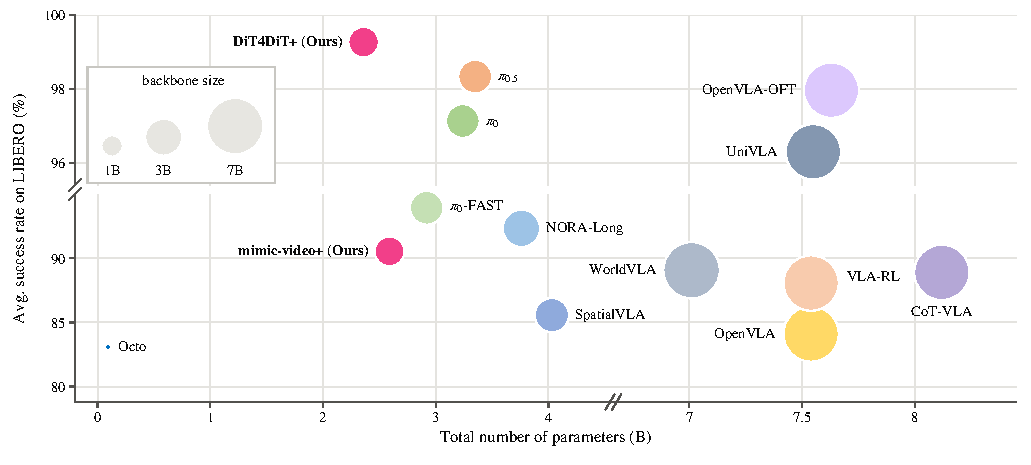
\includegraphics[width=\linewidth]{fig_bubble_params.pdf}
  \caption{\textbf{Performance versus model size on LIBERO.}
  Points show three-suite mean success; the horizontal axis is total parameter count and circle area represents backbone size.
  Our points use 20\% of mimic-video's future tokens and 589/784 DiT4DiT tokens.
  The plot uses a selected set of policies and omits frozen instruction encoders from parameter totals; the table above includes the omitted SmolVLA and Cosmos Policy results and both native evaluations.
  This figure does not establish a matched efficiency comparison across architectures.}
  \label{fig:supp_bubble}
\end{figure*}

\fi

\end{document}
